\documentclass[11pt]{article}

% Change "review" to "final" to generate the final (camera-ready) version.
% Change to "preprint" to generate a non-anonymous version with page numbers.
\usepackage[review]{acl}

% Standard package includes
\usepackage{times}
\usepackage{latexsym}

% For proper rendering and hyphenation of words containing Latin characters
\usepackage[T1]{fontenc}
\usepackage[utf8]{inputenc}

% Microtypography optimizations (improves spacing and reduces overflow)
\usepackage{microtype}

% Typewriter font (optional, may be commented out if unavailable)
\usepackage{inconsolata}

% Image inclusion package and path configuration
\usepackage{graphicx}
\graphicspath{{./}{../}}

% Useful packages for mathematical typesetting and clean tables
\usepackage{amsmath}
\usepackage{booktabs}
\usepackage{url}

% If title and author information overflows the allocated space, uncomment
% the following and set <dim> to 5cm or larger:
%\setlength\titlebox{5cm}

\title{Instructions for *ACL Proceedings and Paper Template}

% ----------------------------------------------------------------------
% AUTHOR INFORMATION TEMPLATES
% ----------------------------------------------------------------------
% Choose the appropriate style for your author list:

% Style 1: Authors from the same institution
\author{First Author \and Second Author \\
  Affiliation / Department \\
  Institution / University Name \\
  Address Line / Country \\
  \texttt{\{first.author, second.author\}@example.edu}}

% Style 2: Authors from different institutions (use \And between institutions)
% \author{First Author \\
%   Department of Computer Science \\
%   University A \\
%   \texttt{first@university-a.edu} \\\And
%   Second Author \\
%   AI Research Lab \\
%   Institution B \\
%   \texttt{second@lab-b.org} \\}

% Style 3: Multiple rows of authors (use \AND to start a new row)
% \author{Author One \\ Affiliation 1 \\\texttt{one@domain} \And
%   Author Two \\ Affiliation 2 \\\texttt{two@domain} \AND
%   Author Three \\ Affiliation 3 \\\texttt{three@domain} \And
%   Author Four \\ Affiliation 4 \\\texttt{four@domain}}

% Style 4: Many authors with indexed affiliations
% \author{
%   \textbf{First Author\textsuperscript{1}},
%   \textbf{Second Author\textsuperscript{2}},
%   \textbf{Third Author\textsuperscript{1,2}} \\
%   \textsuperscript{1}Department of Computer Science, University A \\
%   \textsuperscript{2}Center for Data Science, Institution B \\
%   \small{\textbf{Correspondence:} \href{mailto:first@university-a.edu}{first@university-a.edu}}
% }

\begin{document}
\maketitle

\begin{abstract}
This document serves as the official template and instructions for preparing manuscripts submitted to *ACL conferences (ACL, EMNLP, NAACL, EACL, etc.). The abstract must provide a concise, self-contained summary of the general thesis, methodology, key findings, and conclusions of your work. It should not exceed 200 words and must not contain unexpanded acronyms or numbered bibliographic citations. Replace this placeholder text with your actual paper abstract.
\end{abstract}

\section{Introduction}
\label{sec:intro}

This template is configured for preparing papers adhering to the Association for Computational Linguistics (*ACL) style standards. When writing your paper, replace the guideline text across all sections with your original research while maintaining the structure and formatting commands illustrated here.

\subsection{Submission Modes}
The \texttt{acl} package supports three compilation modes via document options:
\begin{itemize}
    \item \textbf{Review Mode (\texttt{[review]}):} Used for initial double-blind submissions. This mode automatically inserts line numbers in the margins and anonymizes author information.
    \item \textbf{Camera-Ready Final Mode (\texttt{[final]} or default):} Used upon acceptance. Omit the \texttt{review} option to produce the final version without line numbers, displaying full author details.
    \item \textbf{Preprint Mode (\texttt{[preprint]}):} Produces a non-anonymous version that preserves page numbers for posting to repositories such as arXiv.
\end{itemize}

\subsection{Paper Length Guidelines}
Standard *ACL page limits are typically:
\begin{itemize}
    \item \textbf{Long Papers:} Up to eight (8) pages of content for review, plus unlimited pages for references, ethical considerations, and mandatory limitations. Accepted papers usually receive one additional page (up to 9 pages) to incorporate reviewer feedback.
    \item \textbf{Short Papers:} Up to four (4) pages of content for review, plus unlimited pages for references and limitations. Accepted papers usually receive up to five (5) pages.
\end{itemize}
All figures and tables in the main text must fit within these content limits.

\subsection{Double-Blind Anonymity}
Review versions must be completely anonymous:
\begin{itemize}
    \item Do not include author names, affiliations, grant numbers, or personal websites.
    \item Avoid self-identifying references such as \emph{``In our previous paper \citep{Gusfield:97}...''}; instead, write in third person: \emph{``\citet{Gusfield:97} demonstrated...''}.
    \item Omit the Acknowledgments section in the review draft.
\end{itemize}

\section{Document Formatting and Layout}
\label{sec:layout}

All manuscripts must use standard \textbf{A4 paper format} ($21\,\text{cm} \times 29.7\,\text{cm}$) set in a \textbf{two-column} layout.

\subsection{Margins and Column Dimensions}
The exact dimensions for the A4 layout are:
\begin{itemize}
    \item Left, right, top, and bottom margins: $2.5\,\text{cm}$.
    \item Column width: $7.7\,\text{cm}$.
    \item Column height: $24.7\,\text{cm}$.
    \item Column gutter (separation): $0.6\,\text{cm}$.
\end{itemize}
All text, figures, and tables must remain strictly inside these margins.

\subsection{Typeface and Font Sizes}
The primary typeface is \textbf{Times Roman} (11pt base font for body text, single-spaced). The standard hierarchy is:
\begin{itemize}
    \item Title: 15pt bold
    \item Author names: 12pt bold
    \item Section headings: 12pt bold
    \item Subsection headings: 11pt bold
    \item Body text: 11pt regular
    \item Captions, abstract, and bibliography: 10pt regular
    \item Footnotes: 9pt regular
\end{itemize}

\section{Mathematical Equations}
\label{sec:math}

Mathematics can be typeset inline using dollar signs, e.g., $f(x) = \sigma(W x + b)$, or as standalone numbered equations using the \texttt{equation} environment:
\begin{equation}
    \label{eq:sample}
    \text{Attention}(Q, K, V) = \text{softmax}\left(\frac{Q K^T}{\sqrt{d_k}}\right) V
\end{equation}
Refer to numbered equations in the text using \verb|\ref{eq:sample}| or \verb|\eqref{eq:sample}|, producing Equation~\ref{eq:sample}. For multi-line derivations, use the \texttt{align} environment provided by \texttt{amsmath}.

\section{Tables}
\label{sec:tables}

Tables should be formatted cleanly without vertical lines. Use the \texttt{booktabs} package commands: \verb|\toprule|, \verb|\midrule|, and \verb|\bottomrule|. 

\subsection{Single-Column Table}
Table~\ref{tab:sample_table} illustrates a standard single-column table centered in the text column. Always position captions above or below consistently (below is standard for *ACL), and ensure all columns have clear headings.

\begin{table}[ht]
    \centering
    \small
    \begin{tabular}{lrr}
        \toprule
        \textbf{Hyperparameter} & \textbf{Baseline} & \textbf{Proposed} \\
        \midrule
        Learning Rate           & $1\times 10^{-4}$ & $3\times 10^{-4}$ \\
        Batch Size              & 32                & 64                \\
        Warmup Steps            & 500               & 1,000             \\
        Hidden Dimension        & 512               & 768               \\
        Attention Heads         & 8                 & 12                \\
        \bottomrule
    \end{tabular}
    \caption{Example single-column table demonstrating clean layout and parameter formatting using \texttt{booktabs}.}
    \label{tab:sample_table}
\end{table}

\subsection{Two-Column (Full-Width) Table}
When presenting wide datasets or extensive results, span both columns using the \texttt{table*} environment (with an asterisk), as demonstrated in Table~\ref{tab:citations}.

\begin{table*}[t]
    \centering
    \begin{tabular}{lll}
        \toprule
        \textbf{Output Type} & \textbf{Natbib Command} & \textbf{Rendered Result} \\
        \midrule
        Parenthetical Citation & \verb|\citep{Gusfield:97}| & \citep{Gusfield:97} \\
        Textual (In-Text) Citation & \verb|\citet{Gusfield:97}| & \citet{Gusfield:97} \\
        Alternative (No Parentheses) & \verb|\citealp{Gusfield:97}| & \citealp{Gusfield:97} \\
        Multiple Citations & \verb|\citep{Aho:72,Gusfield:97}| & \citep{Aho:72,Gusfield:97} \\
        Possessive Citation & \verb|\citeposs{Gusfield:97}| & \citeposs{Gusfield:97} \\
        \bottomrule
    \end{tabular}
    \caption{Citation commands supported by the ACL style files and their corresponding outputs.}
    \label{tab:citations}
\end{table*}

\section{Figures and Sample Images}
\label{sec:figures}

Figures should be high-resolution (vector PDF or high-DPI PNG) and readable when printed in grayscale. Ensure text within figures is legible and roughly matches the document font size. Captions must be placed directly beneath the figure.

\subsection{Single-Column Figure}
To place a figure within a single column, use the standard \texttt{figure} environment with \verb|\includegraphics[width=\columnwidth]{...}|. Figure~\ref{fig:sample_single} provides a sample illustration using one of the template images (\texttt{cf\_compare.png}).

\begin{figure}[ht]
    \centering
    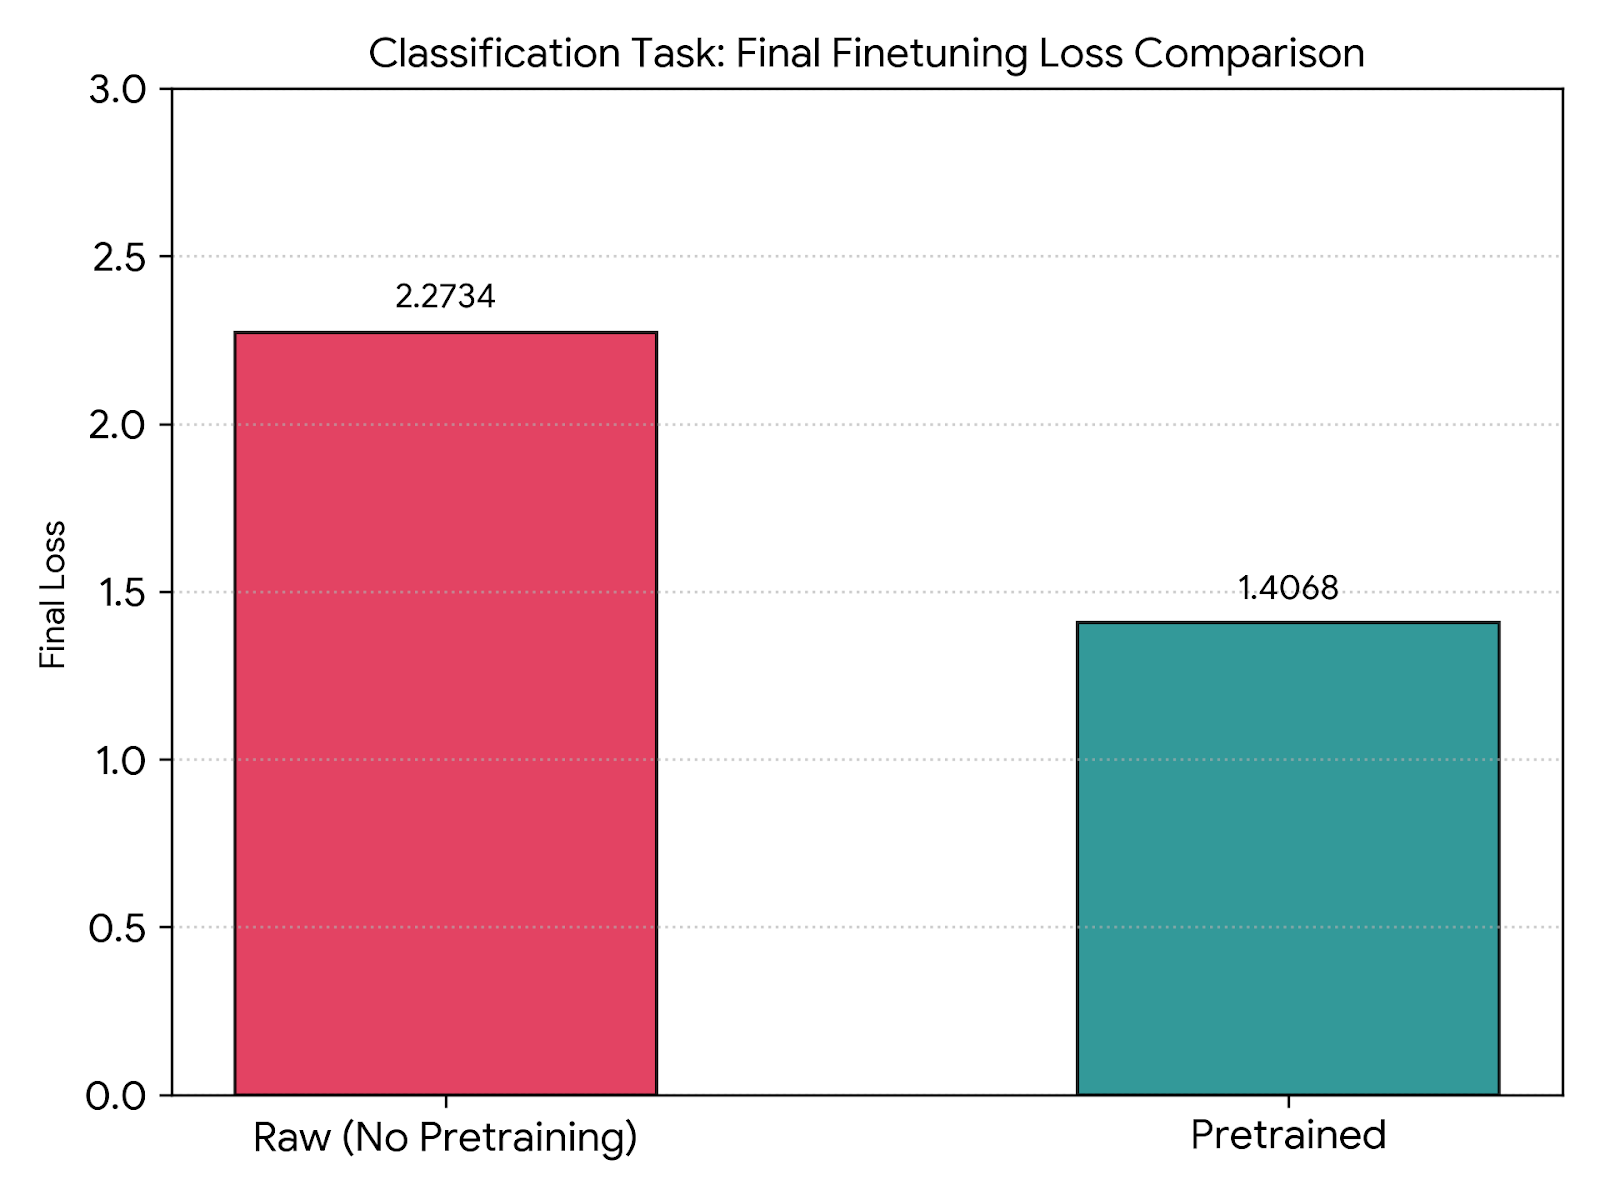
\includegraphics[width=\columnwidth]{cf_compare.png}
    \caption{Sample single-column figure illustrating training/validation loss trajectories. Replace this image file with your own diagram or plot.}
    \label{fig:sample_single}
\end{figure}

\subsection{Wide Two-Column Figure}
For complex visualizations, architectures, or multi-panel plots spanning both columns, use the starred \texttt{figure*} environment. Figure~\ref{fig:sample_wide} illustrates placing two sample images (\texttt{cf\_compare.png} and \texttt{sm\_compare.png}) side-by-side.

\begin{figure*}[t]
    \centering
    \begin{minipage}[b]{0.48\textwidth}
        \centering
        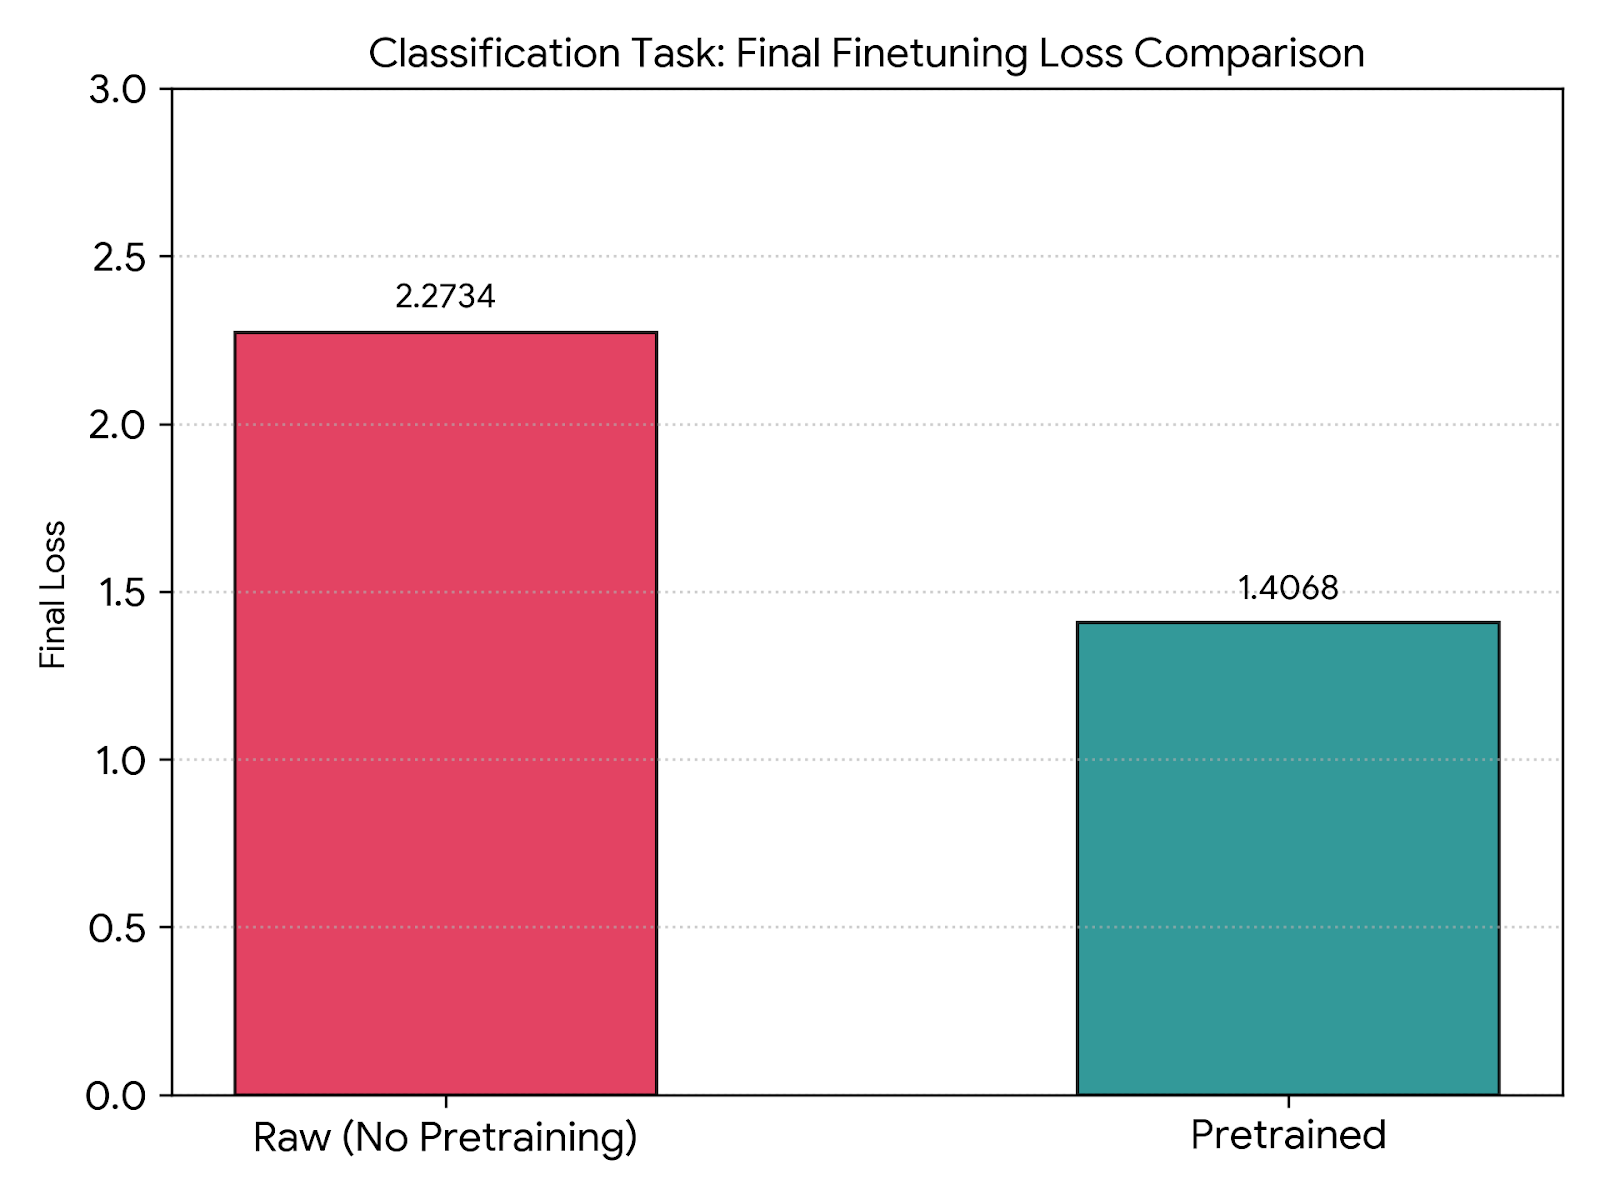
\includegraphics[width=\textwidth]{cf_compare.png}
        \caption*{(a) Experiment A comparison}
    \end{minipage}
    \hfill
    \begin{minipage}[b]{0.48\textwidth}
        \centering
        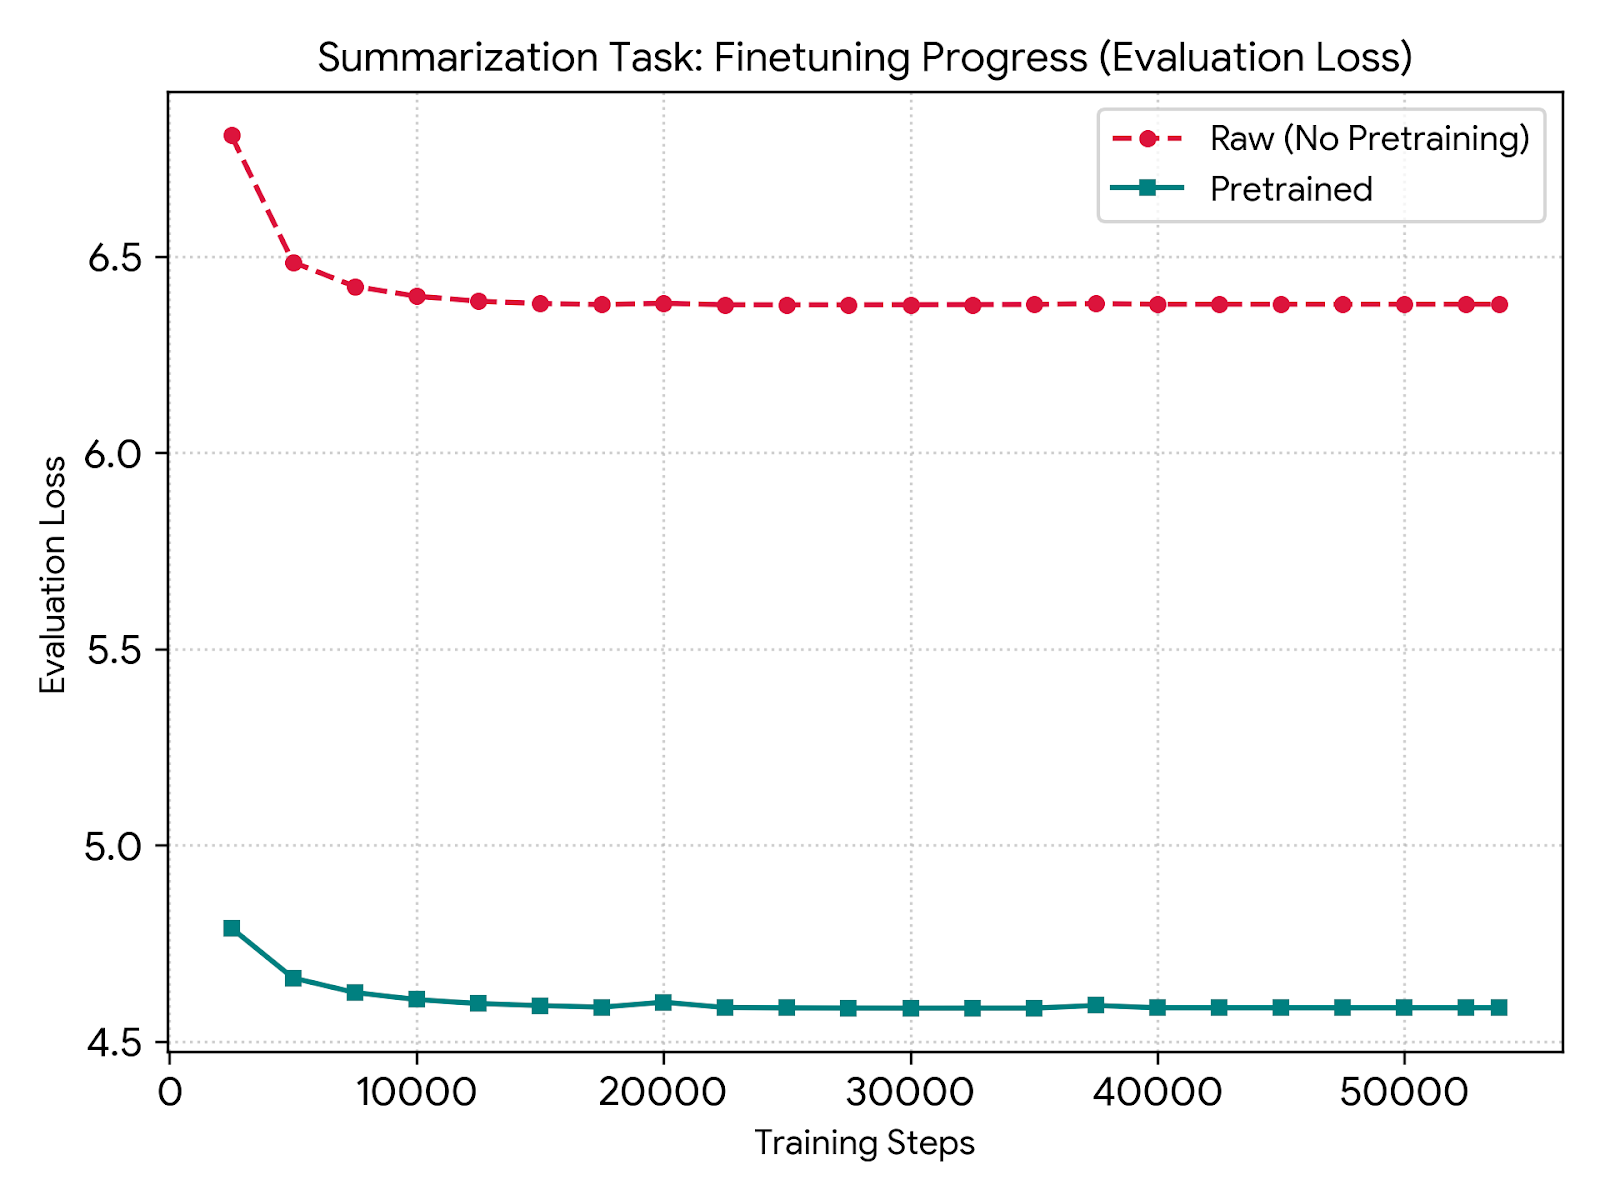
\includegraphics[width=\textwidth]{sm_compare.png}
        \caption*{(b) Experiment B comparison}
    \end{minipage}
    \caption{Sample two-column full-width figure displaying two sub-figures side-by-side using the template sample images.}
    \label{fig:sample_wide}
\end{figure*}

\section{Citations and References}
\label{sec:citations}

Citations are managed via \texttt{natbib} with the custom bibliography style \texttt{acl\_natbib.bst}.

\subsection{Citation Guidelines}
\begin{itemize}
    \item Use \verb|\citep{key}| when the citation is parenthetical, e.g., ``Previous benchmarks have confirmed this trend \citep{Ando2005}.''
    \item Use \verb|\citet{key}| when the author's name forms part of the sentence syntax, e.g., ``As demonstrated by \citet{Vaswani2017}, self-attention mechanisms...''
    \item Never cite using raw brackets or manual numbering.
\end{itemize}

\subsection{Managing Bib\TeX{} Files}
Store non-anthology references in \texttt{custom.bib}. For every entry:
\begin{itemize}
    \item Provide full author names rather than initials wherever available.
    \item Include digital object identifiers (DOIs) via the \texttt{doi = \{...\}} field, or URLs via \texttt{url = \{...\}}.
    \item Wrap capitalized terms, acronyms, and proper nouns in curly braces inside titles (e.g., \verb|{BERT}|, \verb|{GPT}|).
\end{itemize}
To include both your custom citations and the full ACL Anthology bib file, specify:
\begin{verbatim}
\bibliography{anthology,custom}
\end{verbatim}
or specify custom references solely:
\begin{verbatim}
\bibliography{custom}
\end{verbatim}

\section{Footnotes and Links}
\label{sec:links}

Footnotes should be placed at the bottom of the page using the standard command \verb|\footnote{...}|.\footnote{This is an example footnote set in 9pt type.} Footnotes should be separated from the main text by a horizontal rule. Hyperlinks are automatically rendered in dark blue when compiling with hyperref.

\section*{Limitations}
A discussion of limitations is mandatory for *ACL submissions. Authors must explicitly outline the bounds of their study, including potential failure modes, dataset limitations, language coverage, environmental or compute costs, and constraints on generalizability. The Limitations section should be placed after the conclusion and before the references; it does not count toward the page limit.

\section*{Ethics Statement}
Authors are encouraged to provide an ethics statement addressing potential societal risks, biases in data collection or modeling, privacy concerns, and intended use cases. This section does not count toward the page limit.

\section*{Acknowledgments}
Place acknowledgments of funding bodies, collaborators, and computing infrastructure here. \textbf{Important:} This section must be excluded from the initial double-blind review submission and included only in the final accepted version.

% References
\bibliography{custom}

\appendix

\section{Appendices and Supplementary Material}
\label{sec:appendix}

Use \verb|\appendix| before any supplementary sections to switch numbering to alphabetical labels (A, B, C\dots).

Appendices should include supplementary details that are not required for understanding the primary contributions of the paper, such as:
\begin{itemize}
    \item Complete hyperparameter grids and tuning procedures.
    \item Full mathematical proofs and derivations.
    \item Prompts, annotator instructions, and data collection protocols.
    \item Extended qualitative examples and error analysis tables.
\end{itemize}
Reviewers are not obligated to inspect appendices, so the core paper must remain fully self-contained.

\end{document}
